\section{Dettagli Implementativi}

\begin{frame}{Le Fasi}
  \begin{table}
    \renewcommand\arraystretch{1.4}\arrayrulecolor{LightSteelBlue3}

    \begin{tabular}{@{\,}r <{\hskip 2pt} !{\foo} >{\raggedright\arraybackslash}p{5cm}}

      \addlinespace[1.5ex]
      Introduzione     & \small{fase inziale}                                                      \\
      Proposte Attive  & \small{I cittadini possono avanzare proposte}                             \\
      Votazione        & \small{I cittadini votano le proposte  }                                  \\
      Analisi Proposte & \small{L'azienda considera le proposte}                                   \\
      Bilancio         & \small{Viene stanziato un bilancio }                                      \\
      Risultati        & \small{I bilanci vincitori vengono implementati e i cittadini aggiornati} \\
      % \multicolumn{1}{c!{\bfoo}}{} &
    \end{tabular}
  \end{table}
\end{frame}
\begin{frame}
  Le fasi vengono riattivate periodicamente, alla fine di ogni ciclo i cittadini possono fare nuove proposte.


  \begin{center}
    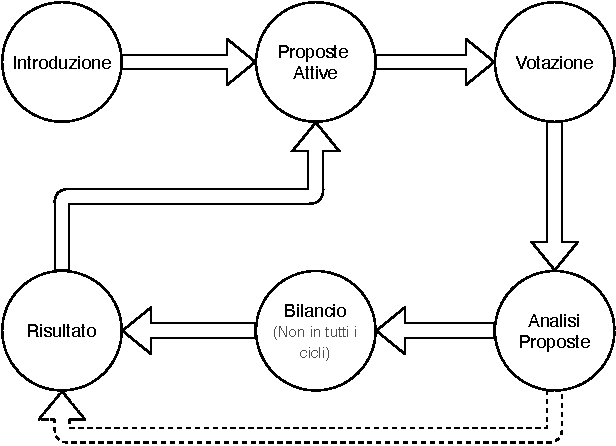
\includegraphics[width=0.7\textwidth]{Fasi}
  \end{center}
  \pause
  L'azienda potrebbe non attivare il bilancio ad ogni ciclo
\end{frame}
